\documentclass[12pt]{article}
\usepackage[a4paper, margin=.30in]{geometry}
\usepackage{graphicx ,
            wrapfig,
            xcolor, 
            enumerate,
            amsmath,fontenc
            }

\newcommand\headerMe[2]{\noindent{}#1\hfill#2}
\renewcommand{\thesection}{\Roman{section}}

\title{Leçon N 6 : Le mouvement}
\author{Zakaria HAOUZAN}
\date{\today}

\begin{document}
% headers --------------
\headerMe{Matière : Physique-Chimie}{Professeur : Zakaria HAOUZAN}\\
\headerMe{Unité : La Mécanique}{Établissement : Lycée SKHOR qualifiant}\\
\headerMe{Niveau : TCS}{Heure : 6H}\\

% ------Content ________
\begin{center}
    \Large{Leçon $N^{\circ}8$: \color{red} Principe d'inertie }
\end{center}


\section{Situation problème : }

\begin{wrapfigure}{r}{0.2\textwidth}
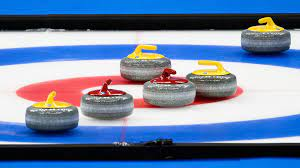
\includegraphics[width=0.2\textwidth]{./img/img00.jpeg}
\end{wrapfigure}


    Après le lancé du palet de curling par un joueur sur le
terrain, on constante que son centre d’inertie garde un
mouvement rectiligne uniforme tant qu’il ne heurte
aucun obstacle.

- Qu’est-ce qu’un centre d’inertie ? Comment trouver sa position ?

- Que s’appelle le palet de curling dans ce cas ?

- Que s’appelle le principe qui peut expliquer cette observation ?

- Est-ce qu’un mouvement nécessite toujours des forces ?

\section{Centre d’inertie d’un corps solide : }
\subsection{Activité 1 }

\begin{wrapfigure}{r}{0.3\textwidth}
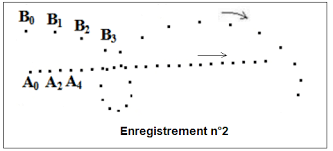
\includegraphics[width=0.3\textwidth]{./img/img01.png}
\end{wrapfigure}


Nous envoyons un autoporteur en rotation sur une table à coussin d’air horizontale équipé de deux éclateurs dont l'une est l’éclateur central qui est fixée au point A et l'autre est fixée au point B, et on obtient l'enregistrement suivant :

1. Comparer les trajectoires de deux points A et B

La trajectoire du B est curviligne tandis que la trajectoire du A est rectiligne.

2. Quelle est la nature du mouvement du point A ? Déduire la nature du mouvement des points de l'axe de la symétrie verticale d’autoporteur passant
par A

La trajectoire de A est rectiligne et que les distances parcourues au cours d'une même
période sont égales, le mouvement du point A est rectiligne uniforme, ceci s'applique
à tous les points de l'axe de symétrie verticale d’autoporteur passant par A .

\subsection{Définition du centre d’inertie G : }

Chaque corps solide a un point spécial et unique appelé centre d’inertie du corps solide et noté G.
Pour les corps homogènes simples il représente le point d'intersection de ses axes de symétrie

\section{Principe d’inertie : }
\subsection{Activité 2}

\begin{wrapfigure}{r}{0.3\textwidth}
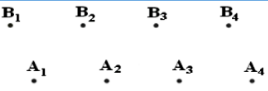
\includegraphics[width=0.3\textwidth]{./img/img03.png}
\end{wrapfigure}


Nous envoyons l’autoporteur sur une table horizontale afin qu'il effectue un
mouvement de translation rectiligne. On obtient alors l'enregistrement
suivant :

1. Comparer le mouvement de deux points A et B. Quelle est la nature du mouvement de G centre d’inertie de
l’autoporteur ?

Mouvements des points A et B rectiligne uniforme, et le mouvement de G centre
d’inertie est aussi rectiligne uniforme, car G appartient à l'axe de symétrie
vertical de l’autoporteur passant par A .

2. Faire l’inventaire des forces appliquées sur l’autoporteur pendant le mouvement. Déterminer la somme
vectorielle de ces forces

Le système étudié : {autoporteur}
Bilan des forces : $\vec{P}$ le poids et $\vec{R}$ la reaction du plan.

Les forces $\vec{P}$ et $\vec{R}$ se compense c-à-d $\vec{P} $=-$  \vec{R}$, alors $\sum \vec{F} = \vec{P} + \vec{R} = \vec{0} $.
 
Nous disons que l’autoporteur est pseudo-isolé mécaniquement parce que la
somme vectorielle de ces forces est nulle.

\subsection{ Système isolé et pseudo-isolé :  }
-Un système est mécaniquement isolé s'il n'est soumis à aucune force. Ce genre de système n'existe pas en pratique (il y a toujours le poids du système et les frottements).

-Un système est pseudo-isolé si la somme vectorielle des forces extérieures auxquelles il est soumis est nulle :
$$\sum \overrightarrow{F_{ext}} = \vec{0}$$

\subsection{Enoncé du principe d’inertie : }

Dans un référentiel galiléen, lorsqu’un solide est isolé ou pseudo-isolé ($\sum \overrightarrow{F_{ext}} = \vec{0}$) ), alors le vecteur vitesse de
son centre d'inertie G est constant : $\overrightarrow{V_G} = \overrightarrow{cst}$

C'est-à-dire :
- Si : le centre d'inertie G est au repos

- Si : le centre d'inertie G est en mouvement rectiligne uniforme

Remarque :
- On appelle repère Galiléen tout repère dans lequel le principe d’inertie est vérifié, on peut considérer que tous les repères liés au sol sont des repères galiléens 

Tout repère en mouvement rectiligne uniforme par rapport à un repère galiléen est un repère galiléen

Le repère lié à un bus en mouvement rectiligne uniforme est un repère
galiléen par Exemple


\section{Relation barycentrique : }
\subsection{Définition de centre de masse d’un système matériel : }

On appelle centre de masse d’un système se constituant de points matériels Ai de masse mi , le barycentre C de ces points. Il est défini par la relation suivante :
$$m_1\overrightarrow{CA_1} + m_2\overrightarrow{CA_2} + ....+ m_n\overrightarrow{CA_n} = \overrightarrow{0}$$

$$\sum m_i\overrightarrow{CA_i} = \overrightarrow{0}$$
N.B : Le centre de masse C d’un système matériel est confondu avec le centre d’inertie G ce système


\subsection{Relation barycentrique : }
\begin{wrapfigure}{r}{0.3\textwidth}

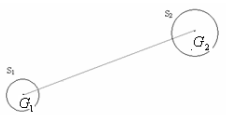
\includegraphics[width=0.3\textwidth]{./img/img04.png}
\end{wrapfigure}
Le centre d’inertie G d’un système composé des corps solides homogènes (Si) de centre d’inertie Gi et de masse
mi est donné par la relation : 
$$\overrightarrow{OG} = \frac{\sum m_i\overrightarrow{OG_i}}{\sum m_i}$$

n : nombre de corps de système.

mi : masse de chaque corps.

Gi : centre d’inertie de chaque corps.

O : point quelconque fixe dans l’espace.

\section{ Exercice d'application : }

On considère un système de deux boules liées par une liaison rigide (voir schéma).
Sachant que $G_1G_2 = 90cm $ et $m_2 = 2 m_1$

déterminer le center d'inertie G du système ($S_1 + S_2$).







\end{document}
